\chapter{簡介}
\renewcommand{\baselinestretch}{10.0} %設定行距
\pagenumbering{arabic} %設定頁號阿拉伯數字
\setcounter{page}{1}  %設定頁數
\fontsize{14pt}{2.5pt}\sectionef

本專題係藉由鋼求平衡台設計,探討協同設計作業之工作模式。

%-------------------研究流程------------------------------%
\section{研究流程}
我們將藉由以下流程探討、研究、並分析協同工具在協同設計上的應用。\\

\begin{figure}[hbt!]
\center
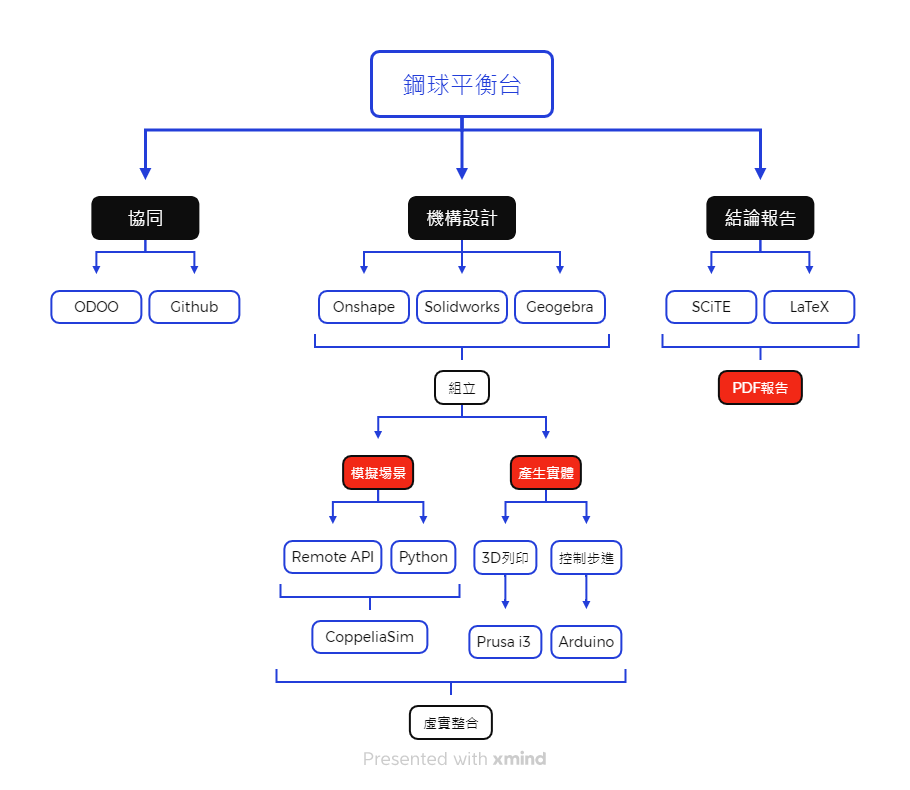
\includegraphics[width=16cm]{0_流程圖}
\caption{\Large 流程圖}\label{0_流程圖}
\end{figure}
\newpage
%-------------------研究環境------------------------------%
\section{專題環境介紹}
\subsection{協同環境}

\subsubsection{(一)ODOO PLM}

ODOO是一個開源的企業管理軟體,旨在幫助公司管理各種業務流程,包括銷售、庫存、會計、製造、資源規劃和人力資源等。
ODOO提供了一個集成的平台,讓用戶可以輕鬆地管理他們的業務活動。
我們將在後面的章節詳細介紹其中的產品生命週期管理(PLM)功能。\\
\begin{figure}[hbt!]
\center

\includegraphics[height=2cm]{odoo}
\caption{\Large odoo 標誌}
\end{figure}

\subsubsection{(二)GitHub}
GitHub是一個基於網絡的程式碼管理和協作平台,為開發者提供了一個集中式的位置來存儲、管理和共享他們的程式碼項目。它使用Git版本控制系統,允許用戶追蹤文件的變更、對其進行版本控制,並輕鬆地進行協作和交流。\\
\begin{figure}[hbt!]
\center

\includegraphics[height=4cm]{github}
\caption{\Large github 標誌}
\end{figure}

\subsection{研究環境}

\subsubsection{(一)Solvespace}
\fontsize{14pt}{2.5pt}\sectionef\hspace{12pt}
Solvespace是一個開源的參數化3D CAD(計算機輔助設計)軟體,旨在幫助用戶創建和編輯3D模型。它具有簡單直觀的用戶界面和豐富的功能,同時還支持多平台運行,包括Windows、Linux和macOS。\\
\begin{figure}[hbt!]
\center
\includegraphics[height=4cm]{Solvespace}
\caption{\Large Solvespace 標誌}
\end{figure}

\subsubsection{(二)Onshape}

Onshape是一個基於雲端的三維計算機輔助設計(CAD)平台,提供了全功能的CAD工具,讓用戶可以通過網絡瀏覽器在任何設備上進行建模和設計。
它的強大功能和靈活性使得用戶能夠輕鬆地創建複雜的三維模型,進行裝配設計、模擬分析以及技術文件繪製等工作。
同時,Onshape的即時協作功能還允許多個用戶同時訪問和編輯同一個設計文件,從而實現更加高效的團隊合作和設計工作流程。\\
\begin{figure}[hbt!]
\center
\includegraphics[height=4cm]{Onshape}
\caption{\Large Onshape 標誌}
\end{figure}


\subsubsection{(三)SolidWorks}
SolidWorks是一款由Dassault Systèmes開發的三維計算機輔助設計(CAD)軟體,廣泛應用於機械設計、工程設計和製造等領域,並且具有強大的建模功能,使得用戶可以快速、精確地創建複雜的三維模型,從而進行裝配設計、渲染、模擬分析等工作。\\
\begin{figure}[hbt!]
\center
\includegraphics[height=4cm]{SolidWorks}
\caption{\Large SolidWorks 標誌}
\end{figure}


\subsubsection{(四)Geogebra}
Geogebra是一款免費的動態數學(幾何)軟體,他的名稱是由\textbf{Geo}metry(幾何)和Al\textbf{gebra}(代數)所組成,主要功能包含CAS計算機、科學計算機、3D計算機、計算與繪圖。
其特點為能建立幾何對象,並保持它們之間的關係,可以用來觀察圖形變化或者製作簡單的動畫、快速的實驗數學上的想法,以製作教學演示材料。\\
\begin{figure}[hbt!]
\center
\includegraphics[height=4cm]{Geogebra}
\caption{\Large Geogebra 標誌}
\end{figure}

\subsubsection{(五)CoppeliaSim}
CoppeliaSim(舊稱V-REP)是由瑞士Coppelia Robotics AG開發的先進機器人模擬器,主要應用於機器人研究和教育。
其支援分佈式控制架構,允許使用Python、Lua和C/C++等語言進行同步和異步控制。內建運動學引擎和多種物理模擬庫,提供精確的運動和剛體模擬。
CoppeliaSim能構建複雜的模型和場景,也能使用插件擴展功能,進行運動規劃及影像處理。\\

\begin{figure}[hbt!]
\center

\includegraphics[height=4cm]{CoppeliaSim}
\caption{\Large CoppeliaSim 標誌}
\end{figure}



\subsection{報告環境}
\fontsize{14pt}{2.5pt}\sectionef\hspace{12pt}
\subsubsection{LaTeX}
\fontsize{14pt}{2.5pt}\sectionef\hspace{12pt}
LaTeX是一種專業的排版系統,通常用於製作科學、技術和學術文檔,如論文、報告、書籍等。與常見的文字處理軟體,和Microsoft Word相比,LaTeX以其強大的排版能力和對數學公式的支援而聞名。

\newpage

\renewcommand{\baselinestretch}{0.5} %設定行距